%\documentclass{acmsiggraph}               % final
\documentclass[review]{acmsiggraph}      % review
%\documentclass[widereview]{acmsiggraph}  % wide-spaced review
%\documentclass[preprint]{acmsiggraph}    % preprint

%% These two line bring in essential packages: ``mathptmx'' for Type 1 
%% typefaces, and ``graphicx'' for inclusion of EPS figures.

\usepackage{mathptmx}
\usepackage{graphicx}

%% use this for zero \parindent and non-zero \parskip, intelligently.

\usepackage{parskip}

%% For code and such.
\usepackage{fancyvrb}
\DefineVerbatimEnvironment{MyVerb}{Verbatim}{fontseries=auto}
\DefineShortVerb{\|}

%% If you are submitting a paper to the annual conference, please replace 
%% the value ``0'' below with your OnlineID. If you are not submitting this
%% paper to the annual conference, you may safely leave it at ``0'' -- it 
%% will not be included in the output.

\onlineid{152}

%% need to document this!

\acmformat{print}

%% Paper title.

\title{Renaissance: A Functional Shading Language}

%% Author and Affiliation (single author).

%%\author{Roy G. Biv\thanks{e-mail: roy.g.biv@aol.com}\\Allied Widgets Research}

%% Author and Affiliation (multiple authors).

\author{Chad Austin\thanks{e-mail:aegisk@cs.iastate.edu}\\ Avatar Factory %
\and Dirk Reiners\thanks{e-mail:dreiners@iastate.edu}\\ Virtual Reality Applications Center\\Iowa State University}

%% Keywords that describe your work.

\keywords{Shading Language, Functional Languages}

%%%%%% START OF THE PAPER %%%%%%

\begin{document}

\maketitle

\begin{abstract}

Programmable graphics hardware is growing in capability and flexibility at a
rapid pace.  Existing languages for programming this hardware force the user
into awareness of hardware architecture (like the separation between vertex
and fragment programs) and make it difficult at best to build collections of
custom graphics algorithms that can be combined as needed.  We present a
pure functional shading language, Renaissance, that uses the concepts of
computational frequency and frequency inference to naturally allow
composition of shader concepts without generating redundant or inefficient
code.  We also provide most of the benefits of metaprogramming languages
without the restriction of requiring a full host environment.

\end{abstract}

%% ACM Computing Review (CR) categories. 
%% See <http://www.acm.org/class/1998/> for details.
%% The ``\CRcat'' command takes four arguments.

\begin{CRcatlist}
 \CRcat{D.3.2}{Programming Languages}{Language Classifications}{Applicative (functional) languages};
 \CRcat{I.3.7}{Computer Graphics}{Three-Dimensional Graphics and Realism}{Color, shading, shadowing, and texture};
 \CRcat{I.3.6}{Computer Graphics}{Methodology and Techniques}{Languages};
\end{CRcatlist}

%% The ``\keywordlist'' command prints out the keywords.
\keywordlist

\section{Introduction}

\copyrightspace

The most important innovation in computer graphics hardware over the last 
decade has been the introduction of programmability. Textures were a first
step  towards fine-grain control over the rendered pixels, and together with
multi-pass  rendering and later multi-textured pipeline configurability they
allowed some  basic implementations of user-specified calculations in the
graphics hardware. But mapping general algorithms to the very limited
and non-intuitive  operations that were possible in this way remained
something of a black art, as  witnessed by the many papers that were
published on mapping specific algorithms to graphics hardware, e.g. 
\cite{heidrich01Shading,kautztowards}. 

Offline rendering for animation had been using much more general languages
for a long time \cite{HanrahanRenderman}, and some attempts were made to map 
them to a slightly extended version of the fixed-function OpenGL pipeline 
\cite{peercy00interactive}. But the real breakthrough came with actual
programs that were executed on the graphics hardware. 

The first steps were assembly languages for GPUs as register machines.
This was a great step forward for generalizing graphics hardware, but
it had its limitations.  Shading algorithms in assembly were not easy
to follow and it was hard to create building blocks of functionality
on which the rest of the shader was built.  The next natural step was
a high-level language built on top of the assembly.  These languages
are similar to C, both in syntax and semantics, or are integrated into
a host language as metaprogramming systems.  These allow tight
integration between the host language and the graphics processor as
well as straightforward shader specialization by using host language
functionality to control shader generation.

Shading languages are beginning to grow features that facilitate
shader composition.  With the advent of Cg's |interface| keyword and
Sh's shader algebra, we're just now starting to see preliminary
support for composable shaders.

In this work we introduce a shading language built on modern
functional languages and their pure functional semantics instead of the
procedural roots currently used. The functional approach significantly
simplifies compilation and analysis of the program, opening up new
avenues for more general optimizations and compositions.

\section{Related Work}

\subsection{Multi-Pass Texture Blending }

Real-time programmable shading appeared in an early form as multi-pass
rendering along with multi-texturing blend modes.  The Quake 3 engine
for example provided a simple shader scripting language to control the
number of passes, texture stages, and rendering states.  This isn't a
complete solution for general shading, but it goes a long way towards
allowing the implementation of several surface appearances, and it allowed
changing shading definitions using a simple text editor without the need to
recompile the program.  Peercy,
Olano et al. discovered that an OpenGL implementation, with some key
extensions, can be treated as a general-purpose SIMD computer in their
OpenGL Shader work \cite{peercy00interactive}.  OpenGL Shader can
support arbitrary shading computation using multiple rendering
passes.

However, current processor trends are leaning towards higher clock rates,
while memory access is slower and higher latency, relatively.  This
precludes large-scale multipass implementations of shading algorithms
from being viable, due to the very high memory bandwidth requirements.
Arbitrary vertex and fragment programs that execute a large set of
instructions per vertex or fragment fit this type of hardware much
more efficiently than multipass approaches to programmability.


\subsection{Assembly Languages (ARBfp, ARBvp, DirectX shader models)}

The next generation of shading languages allowed full programmability at the
vertex and pixel levels via assembly languages for a vector-based register
machine architecture.  Although the instruction sets were limited at first,
the languages allowed arbitrary computation per vertex and per fragment. 
They are more efficient than the multi-pass approaches described above, but
they have obvious disadvantages.  One is that assembly languages are
difficult for people to write and understand, let alone maintain, especially
as programs get larger.  The percieved advantage of assembly languages is
that they are directly executed by the underlying hardware; due to the
variability of graphics hardware, between and even within vendors, this is
rarely the case for shading languages.  Given these limitations, they are
still useful as a compiler backend.


\subsection{Cg, HLSL}

Naturally, the next step beyond an assembly language is a high-level
language that compiles to it.  Cg \cite{mark03cg} and HLSL were
created by NVIDIA and Microsoft, respectively, as C-like, high-level
shading languages.  HLSL compiles to the Microsoft-defined DirectX
vertex and pixel shader models, which are loaded into the card at
runtime.  Cg, on the other hand, compiles to a variety of back ends
and is graphics API-neutral.  The most recent NVIDIA drivers have
support for Cg built in, requiring no manual compilation
step.

When referring to the language originally used by both Cg and
HLSL\footnote{Note that they have since diverged.}, it will simply be called
Cg.  For the sake of compatibility with other shading systems, and
transparent access to the underlying hardware, Cg does very little work for
the user. She is required to specify how data is transferred into the
shaders and which attribute channels map to what. By design, Cg also does
not virtualize any resources, if a feature is not available.  One of Cg's
primary goals is to be as close to the hardware as possible while
maintaining a higher level of abstraction.

Cg and HLSL, while some of the most compelling shading systems for a
variety of reasons, do little to facilitate specialization and
composition of concepts.  Some sort of preprocessor or composition
engine is necessary to reproduce the orthogonality of the fixed
function pipeline.


\subsection{GLSL}

While Cg and HLSL were being developed, 3DLabs and the OpenGL
Architecture Review Board were designing a shading language for the
future of OpenGL.  The OpenGL Shading Language (GLSL \cite{RostGLSL})
had different goals than Cg and HLSL.  It was intended to become part
of the OpenGL standard, replacing the ARB-approved assembly languages.
OpenGL implementers must have the shader compiler in the driver
itself, as opposed to an external process.  This increases driver
complexity, but means that applications that use GLSL benefit from
driver upgrades and compiler improvements for free.  It is also a
forward thinking language design in that it requires all implementers
to support things like conditionals and loops even if they can't do it
in hardware.  It requires virtualization of resources not visible to
the shader writer, such as temporary registers and instruction count.

For the same reasons as Cg and HLSL, GLSL makes a wonderful backend
for a higher-level shading language, but does not provide any
facilities for composable shading itself.


\subsection{RTSL}

Stanford's real time programmable shading system, RTSL \cite{rtsl},
introduced the concept of computational frequency.  They defined four
frequencies: constant, primitive group, vertex, and fragment.
Constant computation is done at shader compile time and not during the
processing of geometry.  Primitive group computation is done per batch
of geometry, while vertex and fragment computations are done per
vertex and per fragment, respectively.  RTSL has a retargetable
backend that can map vertex computation to either the CPU or to basic
programmable vertex hardware.  Fragment computation is mapped to
multi-pass OpenGL, as in OpenGL Shader above, or early fragment
processing hardware like NVIDIA's register combiners.  Their shading
language did not separate vertex and fragment as the compiler was
responsible for splitting the work up among the various computational
stages.  They allowed explicit specification of where computation is
to be done; for example, to easily compare two lighting algorithms,
one per vertex and the other per fragment.

Development of RTSL has halted.  During its development it relied strongly
on multipass rendering, as arbitrary shading calculations were not yet
available in hardware.  Additionally, it is another C-like language
and we are trying to show that a functional language has both
cognitive and implementation simplicity advantages.


\subsection{Sh}

Sh \cite{mccool02shader} isn't exactly a language, per se.  It is a
metaprogramming system on top of C++ designed for building shaders.
Sh is implemented through a set of custom C++ objects that build an
internal program representation when operations are applied to them.
This program is compiled to an underlying shader that is run directly
on the graphics card.  The advantage of a metaprogramming system such
as this is that it has very tight integration with the host
language. If the shader references a global variable, and assignments
are made to that global variable in the host language, outside the
definition of the shader, the data is automatically passed in as a
uniform.  Also, it is natural to use the host language's features in
order to specialize shaders.  For example, if the shader contains an
|if| statement, two different shaders may be generated, based on the
outcome of the condition.

Sh's deal-breaking factor is that it requires a full C++ compiler and
environment.  Thus, shaders can't easily be passed along with 3D
models, limiting their usefulness to people who aren't programmers.
That said, there are some uses for shaders where a metaprogramming
approach is ideal; such as implementation of custom graphics
algorithms tightly bound to the application.


\subsection{Vertigo}

Vertigo \cite{elliott04vertigo} is a metaprogramming system like Sh,
but built on top of Haskell instead of C++.  The interesting aspects
of Vertigo are that it is a functional language and uses expression
rewriting for optimization, which allows it to do an optimal search of
expression space to reduce the amount of computation necessary in a
particular evaluation.  A compelling example is that of vector
normalization, a common operation in graphics programs.  When writing
a function, there is a choice between accepting a normalized vector or
non-normalized vector, which must be normalized explicitly.  Since
normalization is expensive, normalizing a vector twice should be
avoided.  However, in a language with referential transparency it is
possible to take advantage of expression rewriting to reduce the
expression |normalize (normalize v)| to |normalize v|.  Once this
optimization is available, there is no reason not to normalize a
vector, if it needs to be.  Redundant normalize calls are optimized
away.  Vertigo shows how this is done in an elegant and automatic way.

Vertigo suffers from the same problems as Sh, except that it requires
Haskell instead of C++ for shader development.  However, we can take
several of the core advantages of Vertigo, Sh, and RTSL to create a
simpler shading language that enables the same kind of specialization
as the fixed-function pipeline.


\section{Contributions}

% Necessary? DR
% Shading languages have traditionally followed the path of languages for
% general-purpose processors, even when they aren't applicable to the hardware model.  Recent versions of Cg 
% introduce a concept of interfaces, which have syntax and description 
% deceptively similar to interfaces in Java, even though the problem it tries to solve 
% is better addressed by partial evaluation of functional programs and staged computation.

In this paper we introduce a programming language for real-time graphics
hardware that we believe addresses the points necessary for programmable
shading to provide the configurability as the fixed-function pipeline does. 
This language draws from research in modern, pure functional languages, such
as Miranda, Haskell, and Clean.  We base our design on functional languages
for a variety of reasons.  First, functional languages are a very natural
fit to the programming model exposed by graphics hardware.  In the end, all
shaders have to calculate at most three values: a transformed vertex
position, a fragment color and a fragment depth. Everything in the middle is
complication. Using a functional language makes the expressions leading to
these values much more explicit, allowing much cleaner optimizations.
Second, functional languages are traditionally easier to efficiently compile
than imperative languages with side effects, such as C.  Third, our language
is designed to have a minimum of extraneous syntax, making it much easier to
learn and read.

This paper's primary contributions are the following:

\begin{itemize}

\item{A pure functional programming language with a straightforward
  semantic model and syntax}

\item{Automatic computational frequency inference for optimal partitioning
  of program execution to four stages of the graphics pipeline}

\item{Natural shader composability that follows naturally from the simple
  execution model and frequency inference}

\end{itemize}


\section{Key Concepts}

\subsection{Functional Model}

Renaissance is based on the syntax and semantics of modern, typed,
pure functional languages, specifically the family consisting of
Miranda, Haskell, Clean.  Since we don't expect our audience to be
familiar with the syntax or semantics of these languages, the
following will introduce the look and feel with an example.

\begin{MyVerb}
pi = 3.1415927
square x = x * x
circumference r = pi * square r
\end{MyVerb}

The first line defines a name |pi| to have an approximate value of pi.
The second line defines a function called |square| that takes one
parameter and returns its square.  The third line defines the
circumference, given a radius, to be |pi| times the square of the
radius.  |square r| is the syntax for function application, and it
means ``apply the function |square| to the value |r|, substituting the
arguments for the parameters inside the function definition''.  Notice
that the example does not make any types explicit.  Types are inferred
based on a definition's expression and any arguments.  So, above, |pi|
has type |float|.  square's type is |t -> t|, meaning ``a function
that takes type |t| and returns type |t|'', where |t| is the type of
the arguments.  So |square 10| has type |int| and |square 10.0| has
type |float|.  This type inference is discussed in detail later.

There are no loops or variable assignments in this language.  Every
object, once created, cannot be changed.  This is called referential
transparency, which refers to the fact that if the same function
is called twice with the same arguments, the same result will be
returned.

Modern GPUs have a stream programming model: there is a stream of data
elements (vertices or fragments) and a function is applied to all
of them.  This function, in stream programming terminology, is called
a kernel.  Since all of the stream elements are independent, the
function can be run in parallel without any sort of synchronization or
data dependency analysis.  This is largely the reason why graphics
processors these days are so efficient: performance increases linearly
with the number of processors available.  Previous shading languages
have semantic models similar to C; that is, variables that can be
modified and read from.  Furthermore the order in which statements are
executed is critical.  Consider the C-like code in figure \ref{CExample}.

\begin{figure}[htb]
\begin{MyVerb}
int a = 1;
int foo() {
  a += 2;
  // Some code.
  return 10;
}
int bar() {
  a *= 3;
  // Other code.
  return 15;
}
void main() {
  int sum = foo() + bar();
  // do something with a
}
\end{MyVerb}
\caption{C code example}
\label{CExample}
\end{figure}

The value of |a| at the end of |main()| is either 9 or 5, depending on
whether |foo()| or |bar()| is called first.  In general, this
restriction complicates the compiler's task of optimization and static
analysis.  A functional language, on the other hand, is given a lot of
freedom to reorder evaluations, because all dependencies are explicit
and no evaluation has side effects.  For specialized tasks, functional
languages have been shown to perform much more efficiently than
equivalent C code. \cite{ocaml,clean,sac}.

As hardware programmability increases in capability and shaders get
longer and larger, we believe a functional language will scale in both
performance and maintainability more than a language based on the
imperative model of C.  Current shading languages based on C often do,
in fact, compile internally to a single static assignment form and
thus benefit from several of the same optimizations.  This adds a
nontrivial amount of complexity and it makes more sense to start with
a functional model in the first place.

Even ignoring the performance and ``compiler-friendly'' issues,
functional languages are a better mental model for the humans writing
shaders as well.  They make explicit that an operation on a stream
element has no side effects beyond the output value.  Other shading
languages must explicitly document that modifications to global
variables do not affect the program's operation on other stream
elements; conversely, a pure functional language does not even have
the concept of in-place modification, so this kind of confusion is not
possible.


\subsection{Frequency and Type Inference}

% --- It ``smells'' to me like a lot of this should move into the language description.

Renaissance is a statically typed language, like C++, other shading
systems, and most pure functional languages.  That is, the type of an
expression is associated with its name, not its value.  However,
Renaissance infers the type of an expression from context, so no types
need be specified explicitly.  Consider:

\begin{MyVerb}
foo a b = a + bar b
bar b = b + 2
result = foo 10 4
\end{MyVerb}

Notice that no types are explicitly specified, except implicitly
through the values of the constant literals.  However, when |result|
is evaluated, |foo| is called with two integers and returns the sum of
the first and |bar| of the second.  The result of this addition is an
integer as well, so the value |result| has type |int|.  Consider the
definition of a function that normalizes a vector:

\begin{MyVerb}
normalize v = v / length v
\end{MyVerb}

The operation of the function is clear even though its argument and
return types are not specified.  This has a surprising side effect:
the |normalize| function actually represents several functions, each
of different type.  Given that division by a scalar and the length
function can operate on multiple types of vectors, normalize will work
with any vector.  This is similar in practice to C++ template
functions.  Note that we explicitly are not using Hindley-Milner
\cite{milner78,damas82} 
inference.  An ad-hoc overloading approach fits better with the
underlying GLSL and vector operations.

Alongside each expression's type, we also maintain a computational
frequency, a concept introduced by Stanford's RTSL.  There are four
frequencies: constant (per compile), uniform (per primitive group),
vertex (per vertex), and fragment (per fragment).  Built-in shader
inputs each have a specified frequency.  For example, |gl_Vertex| has
the frequency |vertex|, while  |gl_FragCoord| has the frequency |fragment|.
If an operation on two expressions that have different frequencies is
performed, the resulting expression usually has the higher of the two.
One exception is the |if| construct: if the condition has constant
frequency, the |if| is evaluated at compile-time, and, if true, the
resulting frequency is the frequency of the |if-true| expression.
Otherwise, it is the frequency of the |if-false| expression.  Another
important lifting rule is that any linear operation performed in the
fragment shader can be lifted to the vertex shader, the result being
interpolated by the linear interpolate units.

Outputs have a required frequency as well.  The |gl_Position| output
has frequency |vertex| and |gl_FragColor| output has frequency
|fragment|.  It is an error to define |gl_Position| to be an
expression with frequency |fragment|.  Outputs must have frequency
less than or equal to their definition.  Now assume that
|gl_FragColor| depends on the normalized, transformed normal:

\begin{MyVerb}
gl_FragColor = dependsOn (
    normalize (gl_NormalMatrix * gl_Normal))
\end{MyVerb}

|gl_NormalMatrix| has frequency |uniform| and |gl_Normal| has
frequency |vertex|.  Thus, the normal transformation can be done on
the vertex processor.  It looks at first glance like the |normalize|
call can be moved up to the vertex processor too, but, since it is a
nonlinear operation and the fragment interpolators linearly
interpolate, the normalization must be done on the fragment processor.
Conceptually, all operations are done on the fragment processor, and
lifted to earlier stages of the pipeline if possible.


\subsection{Single Shader for Both Vertex and Pixel Pipelines}

In contrast with the most popular real-time shading languages today,
Cg, HLSL, and GLSL, we decided to blur the distinction between vertex
shaders and fragment shaders.  One concern raised by NVIDIA in the
design of Cg is that the different processors support different
functionality, and by making the programs explicitly separate, the
differences are made clear\cite{mark03cg}.  However, recent trends
suggest that the vertex and fragment processors will grow closer in
functionality, rather than farther apart. Microsoft's new graphics
standard, the Windows Graphics Foundation (WGF, aka DirectX 10) is
pushing for a unified processor architecture for both the vertex and
fragment parts of the pipeline \cite{blythewgf}. ATI technology has
also recently been issued a patent on a multi-threaded graphics core
that hides the distinction between vertex and fragment units
\cite{atimtpatent,b3datimtpatent}. With this in mind, we feel the
potential confusion caused by executing ``one'' program on two
potentially-different processors (in addition to the CPU) is worth the
benefit in improved shader clarity, maintainability, and optimization.

To mitigate the potential confusion brought about by this approach, we
may allow specification of computational frequency explicitly, as RTSL
does.  If a lower frequency is specified for a result than the values
it depends on (for example, if it is claimed that a result has a
frequency of |vertex| but it depends on the |fragment|-frequency
|gl_FragCoord| value), a compile-time error is raised.  Conversely,
explicitly specifying a higher frequency than would be inferred would
force computation to occur later in the pipeline, which could be a
performance improvement in some (admittedly rare) cases.


\subsection{Shaders As Data Files}

Following the example set by Cg and GLSL, it is critical that shaders
can be treated as data files so that they can travel along with the
models whose surfaces they describe.  Requiring a compilation step
before being able to load or use a shader greatly increases the amount
of time it takes to iterate changes, especially for shader building
tools and people who aren't programmers.  For this reason, the
approach taken by metaprogramming shading systems is infeasible for
many uses of shaders, such as in games and modeling software.  The
convenience of being able to use a fully-featured general-purpose
language for generation of shaders is offset by the requirement of
having a complete C++ or Haskell compiler in order to use them at all.
Further, the basis of functional programming languages, the lambda
calculus, provides a high degree of abstraction and notational
convenience even with a naive implementation
\cite{PeytonFunctional}.  Therefore, we can provide many of the
important features of other high-level languages, such as higher-order
functions and specialization, with a minimum of effort.  Also, Vertigo
shows that an optimizing compiler from a functional language to GPU
architectures is relatively straightforward, especially compared to an
optimizing C compiler.  In short, we believe a ``small'' functional
language with a simple and powerful semantic model can satisfy the
needs of shaders just as well as the metaprogramming systems, without
the requirement of a large host environment.


\subsection{Composition and Specialization}

The single most important requirement for Renaissance is the ability
to reconfigure the shading pipeline efficiently, just as the fixed
function pipeline does, while still having total control over the
operations performed per-vertex and per-fragment.  Automatic frequency
inference enables the compiler to specialize the shader by constant
inputs without the shader developer having to write entirely different
shaders.  These mechanics are discussed in more detail in the
following section.


\section{System Overview}

The Renaissance system is implemented in C++ and split into two
pieces: the language, including its compiler, and the shader
management API.  For simplicity of implementation and to leverage the
extensive design work that went into the OpenGL Shading Language, we
have chosen GLSL as the basis for a large portion of our language.

When the program loads a shader, it is parsed, validated, and type
checked into an intermediate program structure.  The program can then
set the value of any constant inputs.  When the shader is bound, it is
compiled into code that can run on the GPU, optimized for the constant
values that have been set.  This enables efficient specialization and
composition.  The generated code is cached with the constants used to
create it so recompilation is not necessary when switching back and
forth between shader states.

Setting uniforms and attributes does not invoke recompilation, since
their values do not affect the structure of the generated code.

One of the niceties of metaprogramming languages is that the interface
between the host program and the shader is very convenient, since it
can use native data types and structures.  Contrast this with the
OpenGL Shading Language APIs which require querying and managing
uniform indices, and using function names with `warts' to distinguish
between setting different uniform types: glUniform1f vs. glUniform2i
etc.  We can get close to the convenience of a metaprogramming
language by providing custom C++ types that hide the internal data
transfers.  Figure \ref{InterfaceCode} shows a snippet of example C++
that interfaces with the Renaissance system to set inputs and bind
(implicitly compiling and caching) the shader to the graphics
hardware.

\begin{figure}
\begin{MyVerb}
ren::Bool enableBones(program, "enableBones");

enableBones = true;
program->bind();  // Compiles if necessary.

enableBones = false;
program->bind();  // Compiles if necessary.

enableBones = true;
program->bind();  // Does not compile, already done.
\end{MyVerb}
\caption{Example C++ interface to Renaissance}
\label{InterfaceCode}
\end{figure}

The next two sections define the language and the compiler in more detail.

\section{Language Description}

The syntax and semantics of Renaissance are very similar to the languages 
Miranda, Haskell, and Clean.

A program consists of two components: inputs and definitions.  Each is
separated by a newline.  (Renaissance is whitespace-sensitive.)


\subsection{Inputs}

There are three types of inputs, one for each of the first three
computational frequencies: constants, uniforms, and vertex attributes.
Constant values are taken into account at compile time, uniforms at
primitive group time, and attributes per vertex.  Since their type
cannot be inferred, it must be made explicit:

\begin{MyVerb}
constant bool enablePerPixelLighting
uniform mat3 colorMatrix
attribute float temperature
\end{MyVerb}

\subsection{Definitions}

A definition either specifies a value or a function, with the general form:
name (arguments)* = expression

\begin{MyVerb}
value = 2 + 2
function arg1 arg2 = arg1 / arg2
\end{MyVerb}

|value| is a value of type int and function is a function of type
|s * t -> u| (takes two values of potentially different types and returns
the type of dividing the first by the second).  |function|'s return
type is not evaluated until it is called with arguments.  In this
sense, |function| actually refers to a template of possible functions
which are instantiated when called.

Expressions consist of infix operators and function applications.
Precedence of operations is the same as in GLSL.  Operators are
discussed more fully in a later section.

Evaluation of functions is done lazily, as in Miranda, Haskell, and
Clean.  This prevents redundant and inefficient code generation:

\begin{MyVerb}
constant bool doExpensive
choose expensive cheap = 
        if doExpensive then expensive else cheap
gl_FragColor = choose ExpensiveCalculation
                      CheapCalculation
\end{MyVerb}

The arguments to |choose| are only evaluated if necessary; that is, if
|doExpensive| is true at compile time, then only
|ExpensiveCalculation| will be performed.  Otherwise, only
|CheapCalculation| will be performed.  Lazy evaluation is necessary
for optimal specialized code generation.

\subsection{Types}

Following the conventions set by GLSL, we provide the following types:
|bool|, |int|, |float|, and vectors of 2 to 4 elements of each.
(|vec2| is a vector of two floats, |vec3b| is a vector of three bools,
|ivec4| is a vector of four integers, etc.)  There are also three
square, float matrix types: |mat2|, |mat3|, and |mat4|.  Texture
samplers have type |sampler1D|, |sampler2D|, etc. just as in GLSL.

Arrays have type |[t]| where |t| is the type of its elements.  Since
shading hardware does not yet support variable-length arrays, the
length of the array must be specified at |constant| frequency.  In
order to access the i-th element of an array, an array access is
treated as a function and called with parameter |i|.

In Renaissance, just like in GLSL, there are no implicit type conversions. 
|2 + 2.0| is a type error, requiring a constructor conversion: 
|float 2 + 2.0|.


\subsection{Built-In Functions, Operators, and State}

As with types, we provide access to all GLSL built-in functions, with
the same names, types, and overloads.  Texture access is done as in
GLSL, with the exception that sampler types may be called as functions
with the lookup coordinates as the parameter.

All of GLSL's built-in infix operators are available in Renaissance,
with the same precedence.  Function calls have the highest precedence,
but parentheses are available and operate as expected.  A new |++|
operator is defined as vector concatenation, replacing GLSL's vector
constructors.  Given two floats, concatenating them with |++| returns
a 2-element vector.  For example, |(vec3 1.2 3.4 5.6) ++ 7.8|
evaluates to |(vec4 1.2 3.4 5.6 7.8)|

All GLSL state is exposed in Renaissance as expected, with the
exception of |gl_Color|.  In GLSL, |gl_Color| has a different meaning
in the vertex and fragment programs.  We have simply split its two
meanings into separate names.


\subsection{Overloading and Swizzling}

Renaissance supports what is known as ad-hoc polymorphism, or
overloading, based on the number and type of arguments.  For example,
the expressions |vec4 1.0| and |vec4 1.0 1.0 1.0 1.0| are equally
valid and have the same result, since the first is an overloaded
constructor that fills the vector with its one argument.  There is a
built-in |length| function which takes a vector of any vector type and
returns its length.  Renaissance defines a special dot operator (|.|)
(similar to the language Nice) that calls the right hand side with the
left hand side as its argument.  This means |length vec| and
|vec.length| are equivalent.  This has the nice property that vector
swizzling (|vec.xyz|) can be defined entirely within the standard
library, although, for performance reasons, it is special-cased.


\subsection{Composability}

As developers begin to replace the entire fixed function pipeline with
their own shading algorithms, the restriction that shaders must
replace the entire pipeline becomes an increasing problem.  Moreover,
it is nontrivial to write two independent pieces of the shading
algorithms and combine them into one shader at runtime, even if they
are independent in definition.  Some have solved this problem with
elaborate preprocessors that combine the pieces into one shader that
does not do any redundant computation.  Valve's Half-Life 2, for
example, builds over 1500 shaders as part of their build process by
combining pieces of them with a preprocessor.

As a consequence of the functional programming model and frequency
inference, Renaissance naturally supports composition, as demonstrated
by the following example code:

\begin{MyVerb}
constant bool useLightingModel1
lightModel1 = ...  # calculations for light model 1
lightModel2 = ...  # calculations for light model 2
gl_FragColor = if useLightingModel1 then lightModel1 
                                    else lightModel2
\end{MyVerb}

Since the variable |useLightingModel1| has constant frequency, it is
evaluated at shader compilation time.  Thus, the shader is specialized
based on its value, with no extra computation per fragment.


\subsection{Abstraction Facilities}

Traditionally a vertex program that applies skeletal animation bone
transformations to each vertex looks something like this:

\begin{MyVerb}
uniform [mat4] bones
attribute vec4 boneIndices
attribute vec4 weights

v0 = weights.x * ((bones boneIndices.x) * gl_Vertex)
v1 = weights.y * ((bones boneIndices.y) * gl_Vertex)
v2 = weights.z * ((bones boneIndices.z) * gl_Vertex)
v3 = weights.w * ((bones boneIndices.w) * gl_Vertex)
vertex = v0 + v1 + v2 + v3
gl_Position = gl_ModelViewProjectionMatrix * vertex
\end{MyVerb}

This program has much duplicated logic and is hard-coded for the
number of bones applied to each vertex.  One improvement would be to
use a for loop or iteration construct to iterate over the bone
references.  This would reduce the duplicated logic, but compilers for
these languages do not claim to unroll loops and may even cause the
shader to be virtualized onto the CPU if loops aren't supported by the
underlying hardware.  Given frequency inference and
higher-order-functions, however:

\begin{MyVerb}
constant bool enableBones

uniform [mat4] bones
attribute vec4 boneIndices
attribute vec4 weights

apply i = (weights i) * (bones (boneIndices i))
          * gl_Vertex
skinnedVertex = 
    sum [(apply i) for i in (range 0 3)]
vertex = if enableBones then skinnedVertex else gl_Vertex
gl_Position = gl_ModelViewProjectionMatrix * vertex
\end{MyVerb}

% worth keeping?

The syntax |[expr for var in list]| is called a list comprehension.  A
new list is created by evaluating |expr| on every item in |list|.  In
this case, the new list contains weighted vertices, which must be
summed to get the result.  The sum function takes a list and returns
the result of adding all its elements.  Since the length of the list
has constant frequency, it is automatically unrolled.

It may seem strange that the vector |weights| is being called as a
function, with an index as a parameter.  But, since the index has
|constant| frequency, |weights 0| is compiled into |weights.x|,
|weights 1| is compiled into |weights.y|, etc...

This version of the shader provides a simple switch to enable and
disable bone application at compile time.

\section{Runtime Description}

\subsection{Compiler Backend}

As mentioned above, we are building Renaissance upon GLSL.  It is a
strong foundation for our functional language.  Also, several
functional languages compile to C as it makes a very effective
portable assembly language.  Nothing in the language itself prevents
other backends from being added in the future, however.

Shaders have special output definitions that are the ones actually
responsible for generating code.  |gl_Position| must be defined, for
example, with type |vec4| and frequency of |vertex| or less.  Its
evaluation becomes part of the vertex program.  There are built-in
outputs for the vertex stage, but their definition is optional.  (In
GLSL, vertex programs must output at least a position.)
|gl_FragColor| has the same restriction for |fragment|-frequency
outputs.

\begin{figure}[htb]
\begin{MyVerb}
# Switches.
constant bool EnableLighting

# Uniforms.
uniform vec3 LightPosition
uniform vec3 BrickColor
uniform vec3 MortarColor
uniform vec2 BrickSize
uniform vec2 BrickPct

# Constants.
SpecularContribution = 1.0

# Transform.
gl_Position = ftransform
ecPosition = (gl_ModelViewMatrix * gl_Vertex).xyz
tnorm = normalize (gl_NormalMatrix * gl_Normal)

# Lighting.
lightVec   = normalize (LightPosition - ecPosition)
reflectVec = reflect (-lightVec) tnorm
viewVec    = normalize (-ecPosition)

s = pow (max (dot reflectVec viewVec) 0.0) 3.0
spec = if (diffuse > 0.0) then s else 0.0

LightIntensity = SpecularContribution * spec

# Brick.
origposition = gl_Vertex.xy / BrickSize
condition = fract (origposition.y * 0.5) > 0.5
xoffset = if condition then 0.5 else 0.0
position = origposition + vec2 xoffset 0.0

useBrick = step (fract position) BrickPct

lightFactor = if EnableLighting then
              (LightIntensity + 0.2) else 1.0
amount = useBrick.x * useBrick.y
mixed = (mix MortarColor BrickColor amount)
color = mixed * lightFactor

gl_FragColor = color ++ 1.0
\end{MyVerb}
\caption{Modified brick shader with a lighting toggle 
}
\label{BrickShader}
\end{figure}

\begin{figure}
\begin{center}
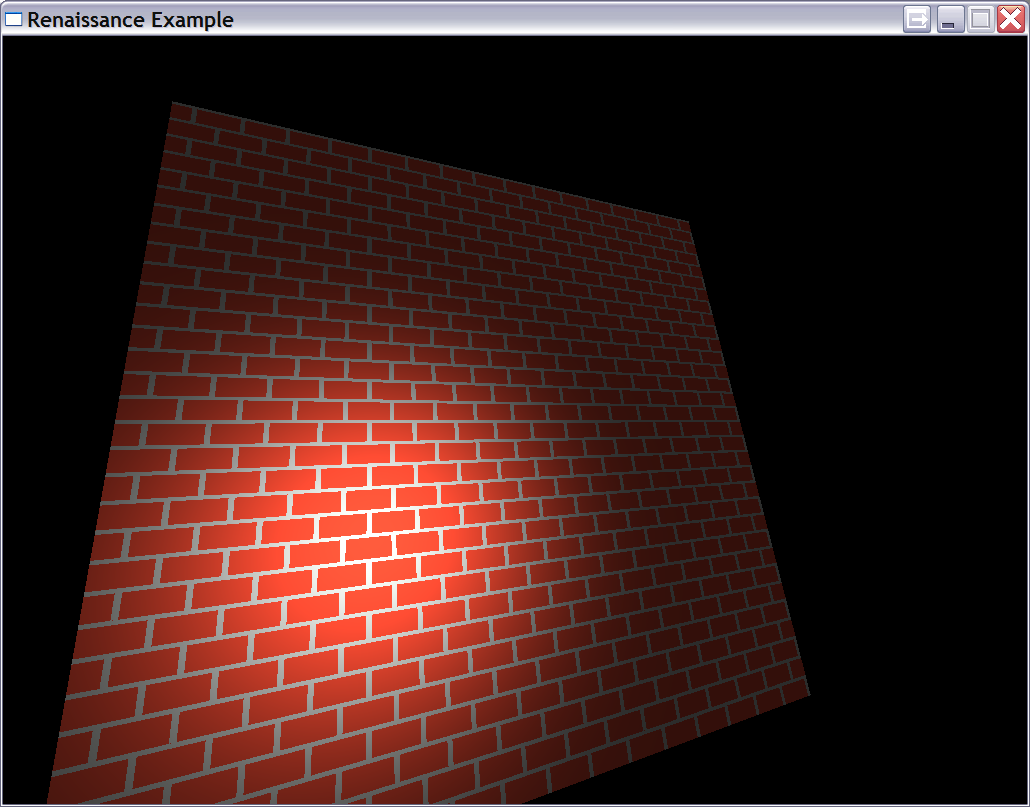
\includegraphics[width=2.3in]{bricklit.eps}
\caption{Lit brick shader}
\end{center}
\label{BrickLit}
\end{figure}

\begin{figure}
\begin{center}
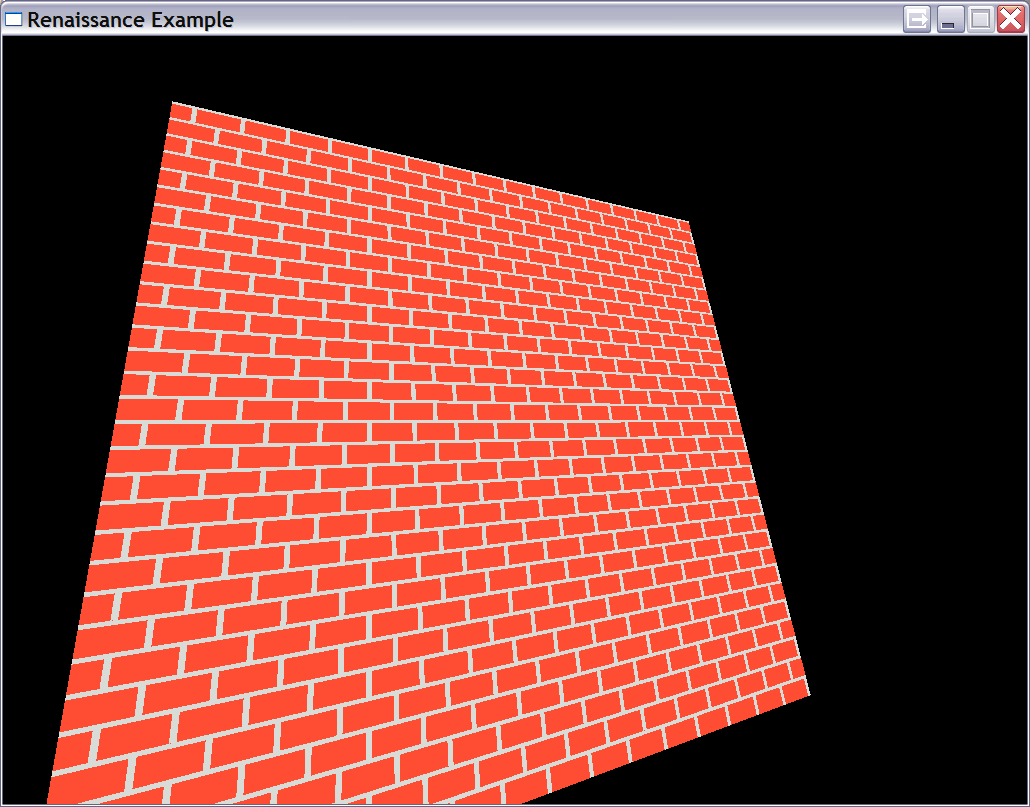
\includegraphics[width=2.3in]{brickunlit.eps}
\caption{Unlit brick shader}
\end{center}
\label{BrickUnlit}
\end{figure}

Fig. \ref{BrickShader} shows the standard OpenGL brick shader
translated directly into Renaissance.  Fig. \ref{BrickLit} shows the
output when lighting is enabled and Fig. \ref{BrickUnlit} shows a
rendering without lighting.  When the constant input |EnableLighting|
is set to false, none of the lighting calculations are performed in
the generated code.

\section{Implementation Status}

A prototype of the system has been developed and can correctly compile
a significant portion of the language.  Most GLSL shaders can be
ported directly to Renaissance.  Our focus has been on the important
optimizations, such as constant evaluation and frequency inference with
expression lifting, instead of low-level generated code work.  We
intend to continue development of Renaissance under an open source
license.


\section{Future Work}

While Renaissance satisfies our expectations, there are clearly areas
that we feel we could improve it.  First, composition and
specialization of shaders in our system requires that everything is
written and compiled in one file.  A ``linking'' or ``module'' system
would allow users to write independent concepts by themselves and then
combine them as needed.  Similarly, we would like to extend the
concept of functional graphics up to the level of multi-pass effects
and state specifications.  As Vertigo \cite{elliott04vertigo} shows so
eloquently, functional programming is a perfect fit for many concepts
in computer graphics.

Our research was focused on implementing high-level optimizations such
as specialization without redundant code.  We would like to apply
Vertigo's expression rewriting system so that we can generate
efficient code at the instruction level as well.  Along the same
lines, additional backends for the assembly language shading languages
are an obvious improvement.

Since a functional language provides a clear, unambiguous
specification of the dependencies in the pipeline, implementing shader
debugging and virtualization on top of Renaissance is a nice
opportunity.

Finally, and most importantly, we would like to use Renaissance to
develop an entirely shader-driven alternative to the fixed function
pipeline.  This would enable shader developers to start with the fixed
function pipeline and customize pieces as needed, rather than starting
completely from scratch every time.  This also would serve as a proof
of concept for Renaissance's design.


\section{Conclusion}

As programmable graphics hardware becomes more prevalent and
instruction and memory limitations are lifted and removed, a next
generation shading language will need to reduce the complexities
associated with transferring data and calculations from the host
application all the way down to the pixels on the screen.

This paper describes Renaissance, a shading language for modern
programmable GPUs that, through the benefits of functional
programming, enables efficient and clear algorithm specifications
across multiple stages of the graphics pipeline.  Through a simple
semantic model and frequency inference, natural composability of
shading ``concepts'' is possible, which existing languages make
difficult at best.  Extending this simple concept, we can imagine a
programmable shading system with configurable state that can be
flipped on and off, just like the interface to the fixed function
pipeline.

\section{Acknowledgments}

We would like to thank Conal Elliot for his work on Vertigo while at
Microsoft Research -- without it we would not have gotten far.  Thanks
also goes to Simon Peyton-Jones at Microsoft Research for his work on
the Haskell language and for releasing his out-of-print book The
Implementation of Functional Programming Languages.  Finally, Dusty
Leary and his infectious love of functional programming greatly
influenced the design of the language.

\bibliographystyle{acmsiggraph}
%\nocite{*}
\bibliography{cits}

\end{document}
